\documentclass[11pt,a4paper]{article}
\usepackage[utf8]{inputenc}
\usepackage[english]{babel}
\usepackage{amsmath}
\usepackage{amsfonts}
\usepackage{amssymb}
\usepackage{graphicx}
\author{Alejandro García Peláez}
\title{EOS Documentation}
\begin{document}

\maketitle 
\break


\vspace*{-3cm}
\section*{Strandbeest Mechanism}

The Jansens Linkage, is an eleven-bar mechanism designed by Theo Janssen who studied physics at the Delft University of Technology but he left the university without a degree; the first "Strandbeest" that the autor created was in 1990, which are moving kinetic structures (wind-propelled).

\noindent\newline The mechanism has some parts in order to get the recognized movement. It can be see in the next picture: \newline \newline

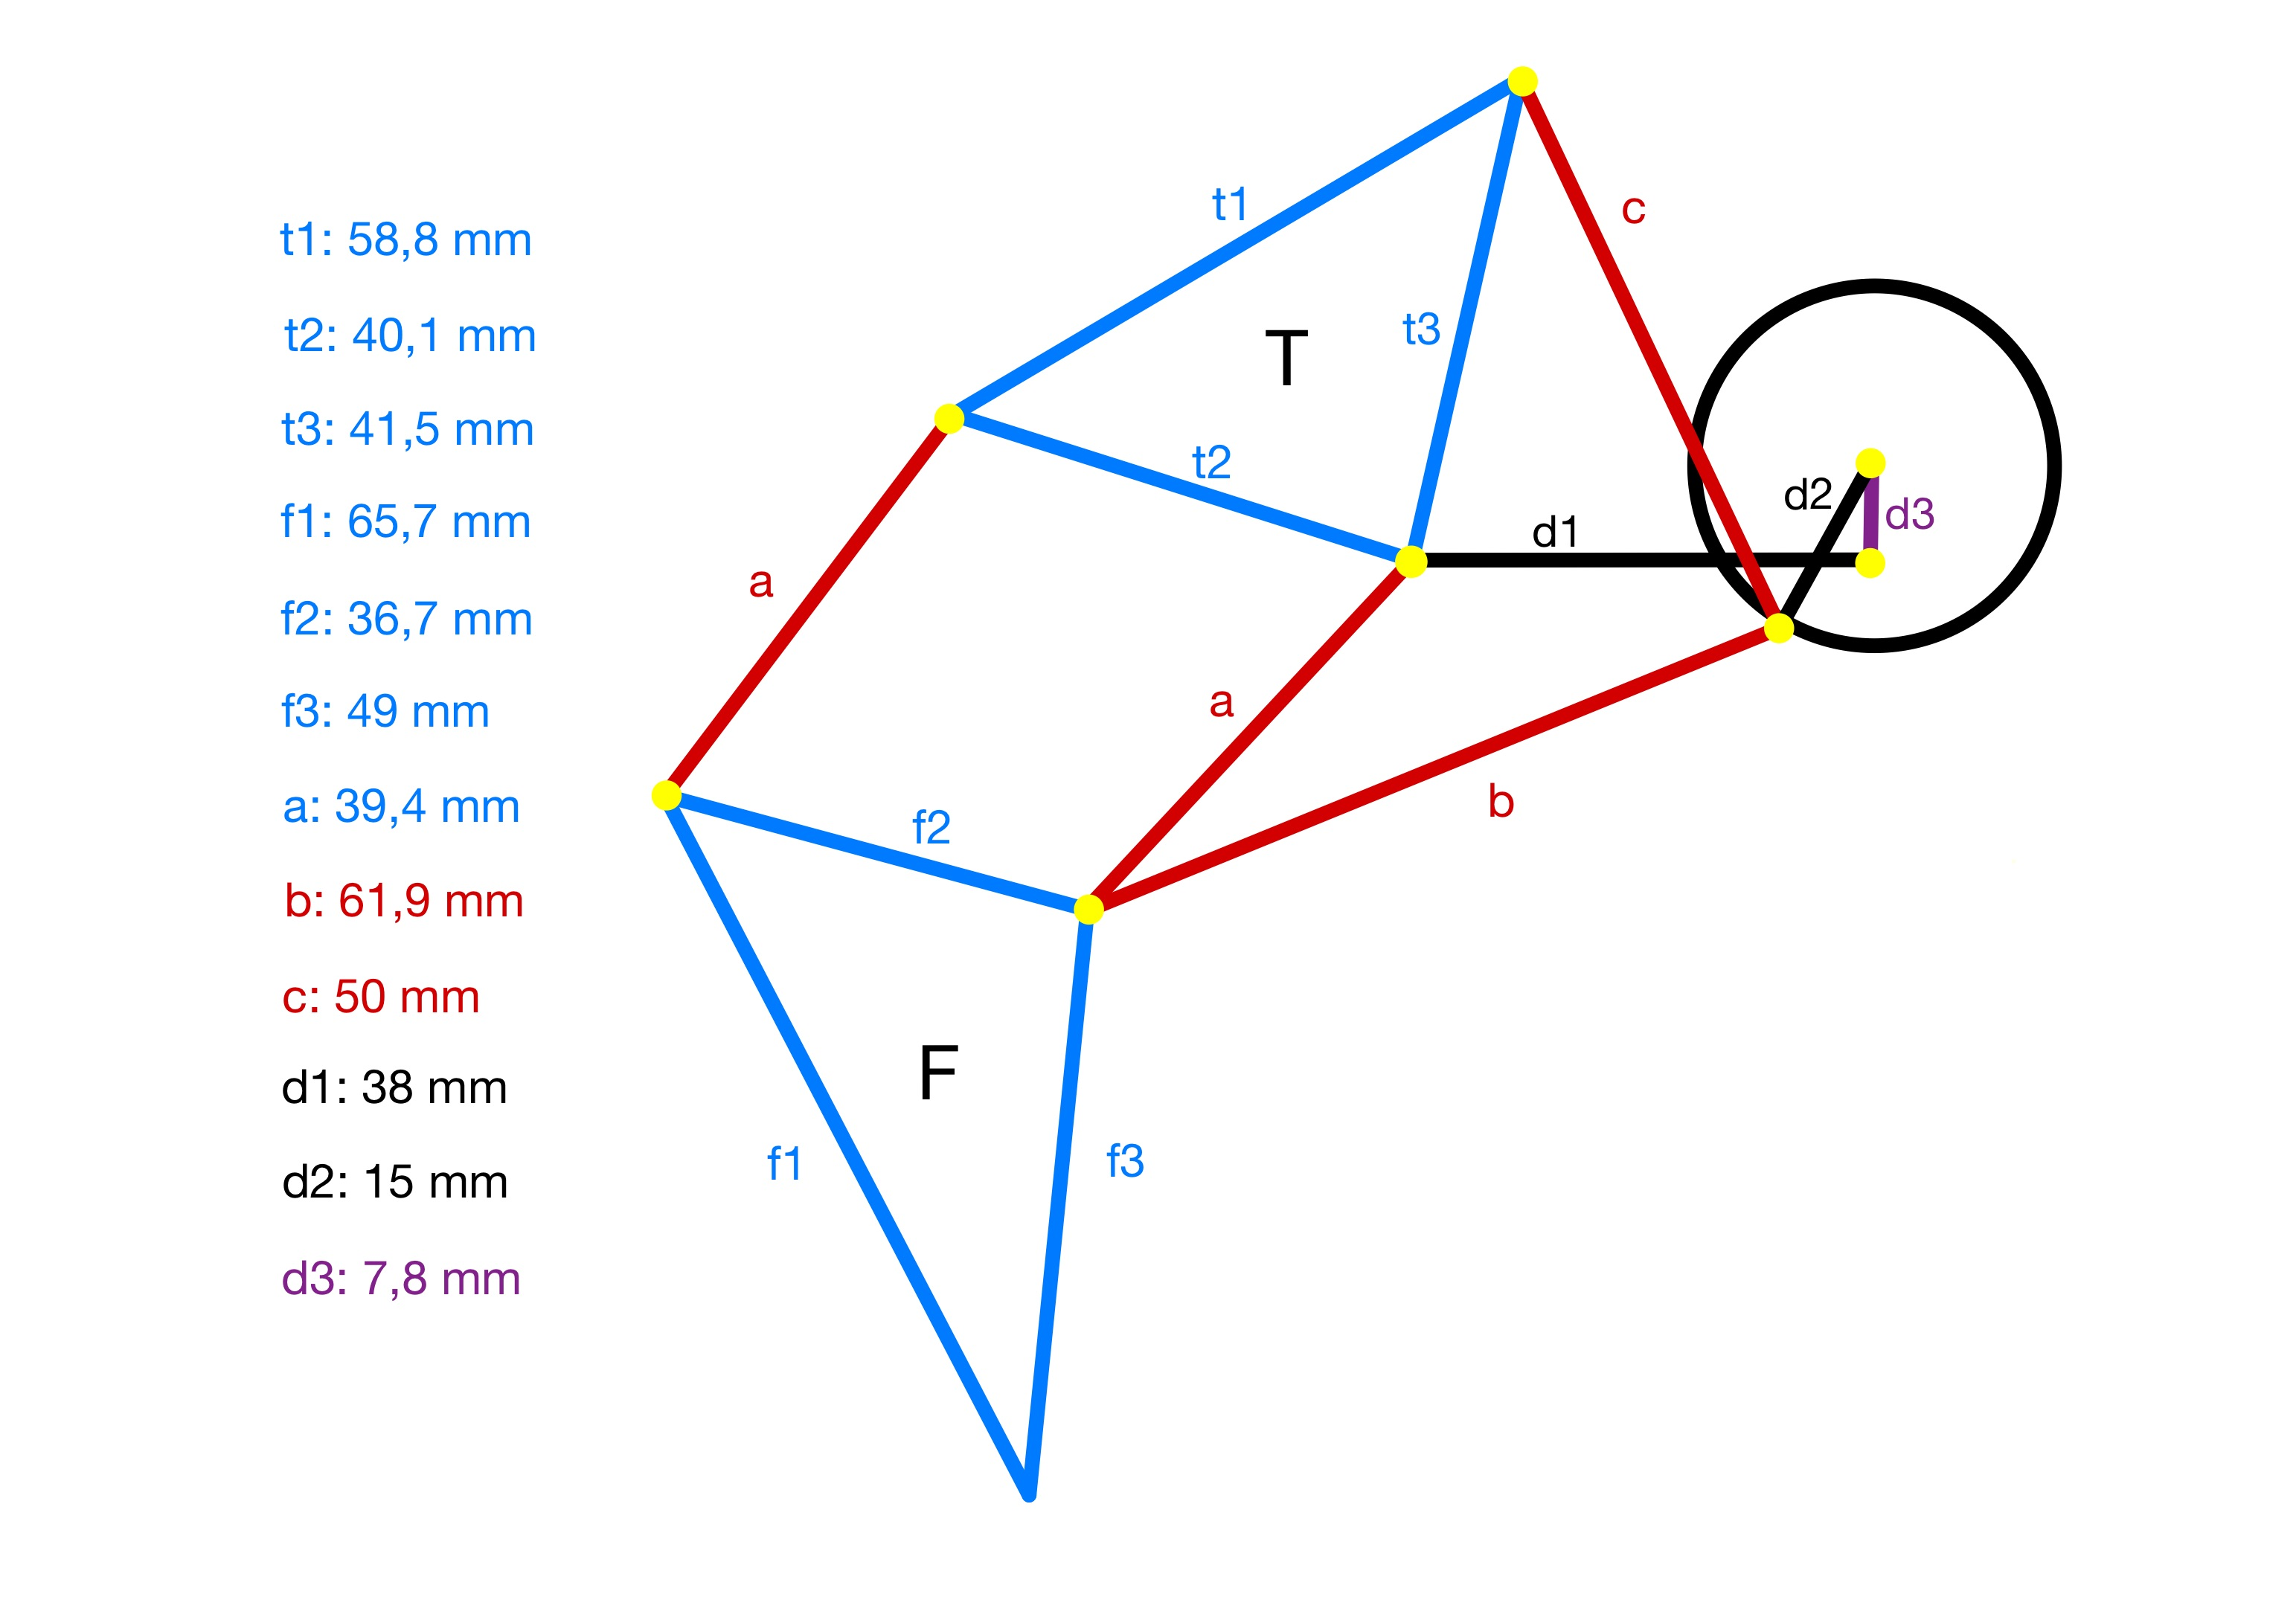
\includegraphics[scale=0.1]{"project_pictures/measures.jpg"}







\end{document}